
\section{Sine models} 

\subsection*{Take a deep breath}

It's that time of semester.  Exams, papers, projects, and all due soon.  And it doesn't help that Halima struggles with executive functioning.  Breaking all those big tasks into smaller, more manageable pieces?  That's a project in itself. Halima sits at her desk and takes nice deep and calming breaths. ``You got this,'' she says to herself.  ``Just breathe in and breathe out.''

Halima feels more centered and sets a timer for 45 minutes to start working on her math project. The professor asked them to pick something from daily life and find an equation that describes it.  Last week she had no idea what to pick, but now it comes to her -- her breath!  She wonders: how could I write an equation that shows how I breathe?

The models Halima has seen so far like linear or exponential have graphs that just go up or down. They are always increasing or always decreasing. That sort of model won't work because the air in her lungs increases (as she breathes in), then decreases (as she breathes out), then increases (as she breathes in), then decreases (as she breathes out), and so on.  Polynomial models have graphs that go up and down a bit, but they don't keep repeating.  How can we write an equation that repeats over and over again?

Halima thinks of many things in her life that repeat. The seasons of the year, waves in the ocean, her hormonal cycle.  So many things.

\subsection*{A sine model}

Wait!  Halima remembers that trig ratios repeat as we go around a circle.  That Ferris wheel her friend Taini was riding.  That revolving door her classmate Aksel keeps talking about.  Those values repeat.  Maybe Halima can model her breathing using a trig function.  

Halima looks up an equation
$$A = 0.4\sin(48T) + 2.3$$
where 
$$A = \text{ volume of air in lungs (in liters) } \sim \text{ dep}$$
$$T = \text{ time since we started measuring lung volume (in seconds) } \sim \text{ indep}$$
and the sine function is set to take inputs in degrees.

She calculates a few values. When $T=0$ the volume of air is
$$0.4 \times \boxed{\texttt{sin}}(48 \times 0) + 2.3= 2.3 \text{ liters}$$
When $T=1$ the volume of air is
$$0.4 \times \boxed{\texttt{sin}}(48 \times 1) + 2.3= 2.5972579302 \approx 2.6 \text{ liters}$$
When $T=2$ the volume of air is
$$0.4 \times \boxed{\texttt{sin}}(48 \times 2) + 2.3= 2.6978087581 \approx 2.7 \text{ liters}$$

Halima makes a table of values for $T=1, 2, \ldots, 10$ seconds and rounds each answer to one decimal place.

\begin{center}
\begin{tabular}{c|c|c|c|c|c|c|c|c|c|c|c}
    $T$ & 0 & 1 & 2 & 3 & 4 & 5 & 6 & 7 & 8 & 9 & 10 \\ \hline
    $A$ & 2.3 & 2.6 & 2.7 & 2.5 & 2.2 & 2.0 & 1.9 & 2.1 & 2.5 & 2.7 & 2.6
\end{tabular}
\end{center}

Halima notices that the air volume goes up, then down, then up as expected.  She decides to extend her table to confirm that the trend continues.

\begin{center}
\begin{tabular}{c|c|c|c|c|c|c|c|c|c|c}
    $T$ & 11 & 12 & 13 & 14 & 15 & 16 & 17 & 18 & 19 & 20 \\ \hline
    $A$ & 2.4 & 2.1 & 1.9 & 2.0 & 2.3 & 2.6 & 2.7 & 2.5 & 2.2 & 2.0 
\end{tabular}
\end{center}

To see what's happening, Halima plots the points.

\begin{center}
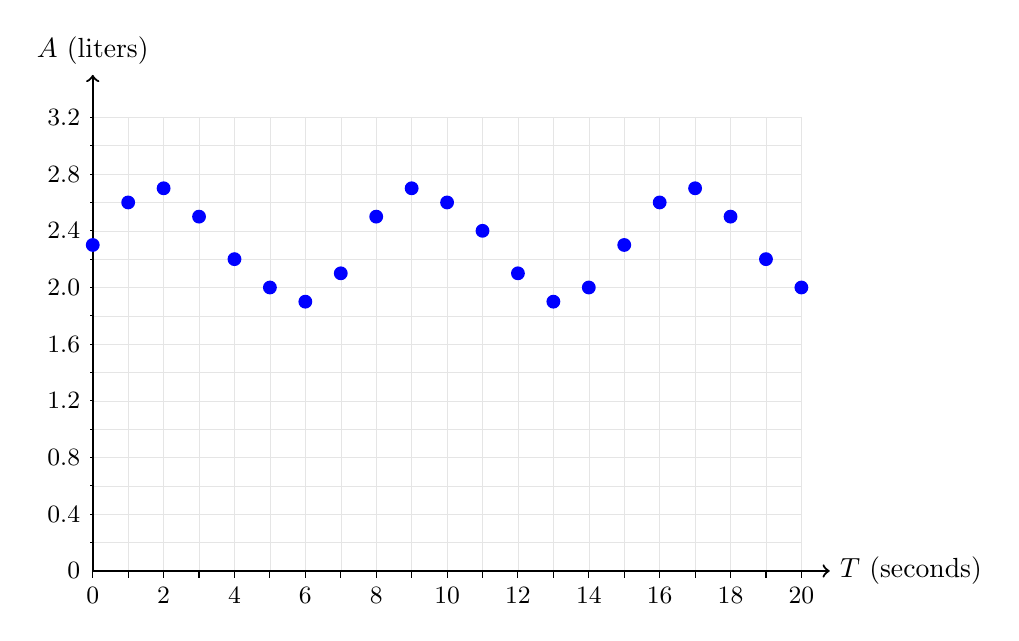
\begin{tikzpicture}[x=0.45cm, y=1.8cm]
  % Grid (x step = 1, y step = 0.2, y max = 3.2)
  \draw[gray!20, very thin, xstep=1, ystep=0.2] (0,0) grid (20,3.2);
  
  % Major axes & labels
  \draw[->, thick] (0,0) -- (20.8,0) node[right] {$T$ (seconds)};
  \draw[->, thick] (0,0) -- (0,3.5) node[above] {$A$ (liters)};
  
  % X-axis ticks at EVERY integer (0 to 20)
  \foreach \x in {0,1,...,20} {
    \draw (\x,0) -- (\x,-0.05);
  }
  % X-axis labels only on EVEN numbers
  \foreach \x in {0,2,4,6,8,10,12,14,16,18,20} {
    \node[below] at (\x,-0.05) {\small \x};
  }
  
  % Y-axis tick marks every 0.2 (0.2 to 3.2)
  \foreach \y in {0.2, 0.4, 0.6, 0.8, 1.0, 1.2, 1.4, 1.6, 1.8, 2.0, 2.2, 2.4, 2.6, 2.8, 3.0, 3.2} {
    \draw (0,\y) -- (-0.08,\y);
  }
  
  % Y-axis labels every 0.4 (0 to 3.2)
  \foreach \y in {0, 0.4, 0.8, 1.2, 1.6, 2.0, 2.4, 2.8, 3.2} {
    \node[left] at (-0.08,\y) {\small \y};
  }
  
  % Data Points (T = 0 to 20)
  \foreach \x/\y in {
    0/2.3, 1/2.6, 2/2.7, 3/2.5, 4/2.2, 
    5/2.0, 6/1.9, 7/2.1, 8/2.5, 9/2.7, 10/2.6,
    11/2.4, 12/2.1, 13/1.9, 14/2.0, 15/2.3,
    16/2.6, 17/2.7, 18/2.5, 19/2.2, 20/2.0
  } {
    \fill[blue] (\x,\y) circle (2.5pt);
  }
\end{tikzpicture}
\end{center}

Next, she draws in a smooth curve.

\begin{center}
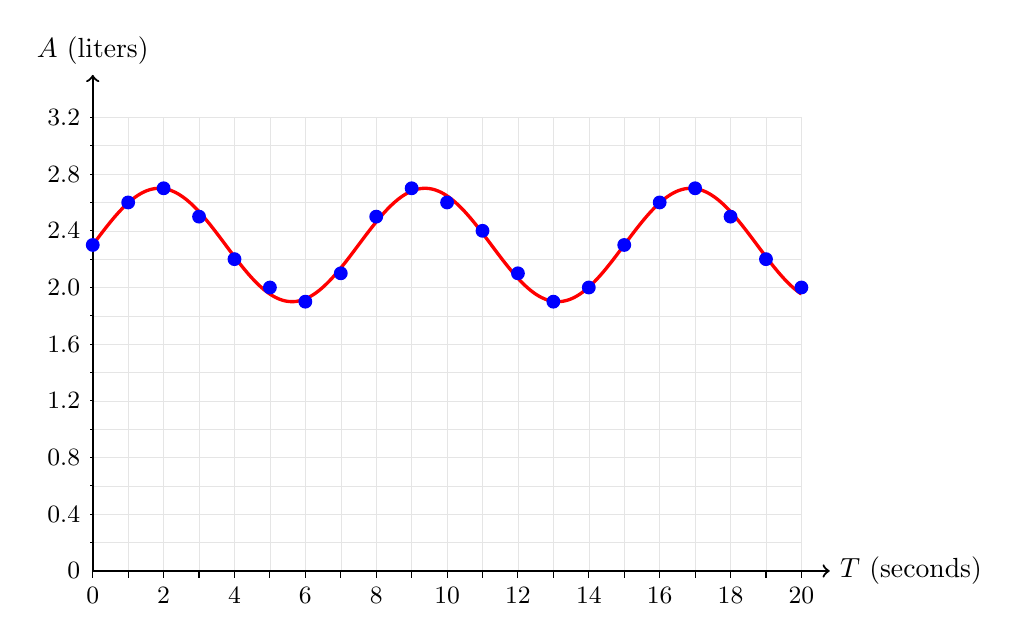
\begin{tikzpicture}[x=0.45cm, y=1.8cm]
  % Grid (x step = 1, y step = 0.2, y max = 3.2)
  \draw[gray!20, very thin, xstep=1, ystep=0.2] (0,0) grid (20,3.2);
  
  % Major axes & labels
  \draw[->, thick] (0,0) -- (20.8,0) node[right] {$T$ (seconds)};
  \draw[->, thick] (0,0) -- (0,3.5) node[above] {$A$ (liters)};
  
  % X-axis ticks at EVERY integer (0 to 20)
  \foreach \x in {0,1,...,20} {
    \draw (\x,0) -- (\x,-0.05);
  }
  % X-axis labels only on EVEN numbers
  \foreach \x in {0,2,4,6,8,10,12,14,16,18,20} {
    \node[below] at (\x,-0.05) {\small \x};
  }
  
  % Y-axis tick marks every 0.2 (0.2 to 3.2)
  \foreach \y in {0.2, 0.4, 0.6, 0.8, 1.0, 1.2, 1.4, 1.6, 1.8, 2.0, 2.2, 2.4, 2.6, 2.8, 3.0, 3.2} {
    \draw (0,\y) -- (-0.08,\y);
  }
  
  % Y-axis labels every 0.4 (0 to 3.2)
  \foreach \y in {0, 0.4, 0.8, 1.2, 1.6, 2.0, 2.4, 2.8, 3.2} {
    \node[left] at (-0.08,\y) {\small \y};
  }

  % Smooth Sine Curve using the mathematical equation A = 0.4*sin(48*T) + 2.3
  \draw[red, very thick, samples=300, domain=0:20] plot (\x, {0.4*sin(48*\x) + 2.3});
  
  % Data Points (T = 0 to 20)
  \foreach \x/\y in {
    0/2.3, 1/2.6, 2/2.7, 3/2.5, 4/2.2, 
    5/2.0, 6/1.9, 7/2.1, 8/2.5, 9/2.7, 10/2.6,
    11/2.4, 12/2.1, 13/1.9, 14/2.0, 15/2.3,
    16/2.6, 17/2.7, 18/2.5, 19/2.2, 20/2.0
  } {
    \fill[blue] (\x,\y) circle (2.5pt);
  }
\end{tikzpicture}   
\end{center}

\subsection*{Understanding the sine model}

Part of Halima's assignment for the project is to describe the meaning of each constant in the equation,
$$A = 0.4\sin(48T) + 2.3$$
What do the 0.4, 48, and 2.3 mean in the story, including their units, and how can we see those numbers in the graph?

In the story, 2.3 liters is the amount of air left in the lungs right before she breathes in (at the end of a normal, relaxed exhalation). The points on the graph go from a high of 2.7 to a low of 1.9.  The value 2.3 is right in the middle, the average.  We say the \textbf{midline} of the graph is at height 2.3 liters.  

Since sine ratios are unitless, 0.4 must also be in liters.  In the equation, the sine term can be as big as +1, in which case we have 
$$.4(1) + 2.3 = 2.7$$
or as small as -1, in which case we have
$$.4(-1) + 2.3 = 1.9$$
In the graph, the distance from the midline to the top peaks (or the distance from the midline to the bottom pits) is 0.4 liters. We say that the \textbf{amplitude} of the function is 0.4 liters.

The 48 is trickier.  Let's start with its units. We know that $48T$ must be in degrees.  Since $T$ is in seconds, the only way it works is if the units for 48 are degrees per second.  Check it out:
$$\frac{48^\circ}{\text{sec}}\times T\text{ sec} = 48T^\circ$$

Normally, the value of sine repeats every time we make a full circle, or 360$^\circ$.  Because the equation has $48T$ as the number we use to evaluate sine, the values will repeat every time $$48T=360$$
Dividing each side of this equation by 48 we get 
$$T = \frac{360}{48} = 360 \div 48 = 7.5$$
The breathing pattern repeats every 7.5 seconds. 

In the graph, we see the distance from one high peak to the next (or from one low pit to the next) is 7.5. We say the \textbf{period} of the sine function is 7.5 seconds. Notice that we do not see 48 directly in the graph; instead, we see $\frac{360}{48}=7.5$.

Halima draws the graph one more time, labeling these new numbers.

\begin{center}
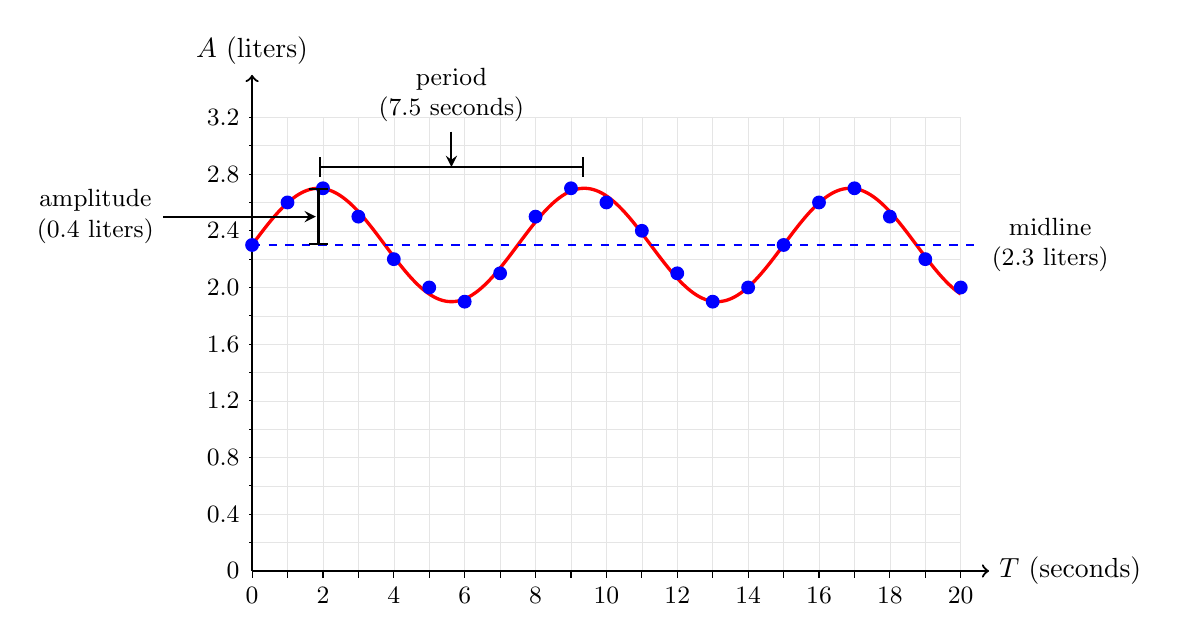
\begin{tikzpicture}[x=0.45cm, y=1.8cm]
  % Grid (x step = 1, y step = 0.2, y max = 3.2)
  \draw[gray!20, very thin, xstep=1, ystep=0.2] (0,0) grid (20,3.2);
  
  % Major axes & labels
  \draw[->, thick] (0,0) -- (20.8,0) node[right] {$T$ (seconds)};
  \draw[->, thick] (0,0) -- (0,3.5) node[above] {$A$ (liters)};
  
  % X-axis ticks at EVERY integer (0 to 20)
  \foreach \x in {0,1,...,20} {
    \draw (\x,0) -- (\x,-0.05);
  }
  % X-axis labels only on EVEN numbers
  \foreach \x in {0,2,4,6,8,10,12,14,16,18,20} {
    \node[below] at (\x,-0.05) {\small \x};
  }
  
  % Y-axis tick marks every 0.2 (0.2 to 3.2)
  \foreach \y in {0.2, 0.4, 0.6, 0.8, 1.0, 1.2, 1.4, 1.6, 1.8, 2.0, 2.2, 2.4, 2.6, 2.8, 3.0, 3.2} {
    \draw (0,\y) -- (-0.08,\y);
  }
  
  % Y-axis labels every 0.4 (0 to 3.2)
  \foreach \y in {0, 0.4, 0.8, 1.2, 1.6, 2.0, 2.4, 2.8, 3.2} {
    \node[left] at (-0.08,\y) {\small \y};
  }

  % Smooth Sine Curve using equation A = 0.4*sin(48*T) + 2.3
  \draw[red, very thick, samples=300, domain=0:20] plot (\x, {0.4*sin(48*\x) + 2.3});
  
  % Data Points (T = 0 to 20)
  \foreach \x/\y in {
    0/2.3, 1/2.6, 2/2.7, 3/2.5, 4/2.2, 
    5/2.0, 6/1.9, 7/2.1, 8/2.5, 9/2.7, 10/2.6,
    11/2.4, 12/2.1, 13/1.9, 14/2.0, 15/2.3,
    16/2.6, 17/2.7, 18/2.5, 19/2.2, 20/2.0
  } {
    \fill[blue] (\x,\y) circle (2.5pt);
  }

  % Dashed horizontal line at A = 2.3 in blue extending past graph edge
  \draw[blue, thick, dashed] (0,2.3) -- (20.5,2.3);

  % Midline label in black to the right of the graph
  \node[right, black, font=\small, align=center] at (20.6, 2.3) {midline \\ (2.3 liters)};

  % Period bar in |--| format between 1st & 2nd peak, with label above pointing down
  \draw[|-|, thick] (1.875, 2.85) -- (9.375, 2.85);
  \node[above, font=\small, align=center] (period_label) at (5.625, 3.1) {period \\ (7.5 seconds)};
  \draw[->, >=stealth, thick] (period_label.south) -- (5.625, 2.85);

  % Amplitude dimension line & two-line label to the left with pointing arrow
  \draw[|-|, thick] (1.875, 2.3) -- (1.875, 2.7);
  \node[left, font=\small, align=center] (amp_label) at (-2.5, 2.5) {amplitude \\ (0.4 liters)};
  \draw[->, >=stealth, thick] (amp_label.east) -- (1.8, 2.5);
\end{tikzpicture}
\end{center}

\input{GoDoWS}

\noindent \textbf{Do you know \ldots}

\begin{itemize}
\item How to make a table and graph of a sine function?
\item What the graph of a sine function looks like?
\item What the period, amplitude, and midline of a sine function mean in terms of the graph and the story?
\item How to determine the period, amplitude, and midline of a sine function from the equation, and what the units are?

 \input{NotSure} 
\end{itemize}

\subsection*{Exercises}

\begin{enumerate}

\item %workbook 1
Sara and her brother Nahiz run a small coffee shop, Qamaria Cafe.  The basement serves as storage and tends to be fairly humid so they run a dehumidifier to remove water from the air. The dehumidifier automatically cycles on and off.  When it turns off, the humidity rises a bit and when it turns back on, the humidity falls again.  The humidity ($H$\%) depends on the time ($T$ hours) where we measure time from 12:00 PM (midnight) when the machine turns on.  An equation describing this dependence is 
$$H = 5\sin(90T)+50$$
where the sine function is set to take inputs in degrees.
\begin{enumerate}
    \item According to the equation, what is the humidity level at midnight? Hint: $T=0$.
    \item Make a table showing the humidity at midnight, 1:00 AM, 2:00 AM, 3:00 AM, 4:00 AM, 5:00 AM, 6:00 AM, 7:00 AM and 8:00 AM.
    \item Draw a graph illustrating the relationship.
    \item What is the average humidity level? Hint: it's the height of the midline of the graph.
    \item How often does the humidifier make a full cycle (on/off)?  Hint: it's the period.
\end{enumerate}

\item %workbook 2

Sara's specialty is lattes -- hot espresso coffee with steamed milk. Qamaria Cafe's monthly latte revenue goes up and down depending on the season.  Based on data from 2025, Sara estimates that 
$$R=6000\sin(30M)+8000$$
where
$$M = \text{ time (in months since October 2025) } \sim \text{ indep}$$
$$R = \text{ latte revenue (in \$) } \sim \text{ dep}$$
and the sine function is set to take inputs in degrees.

Nahiz drew a graph showing three years of expected revenue if Sara's model continues.

\begin{center}
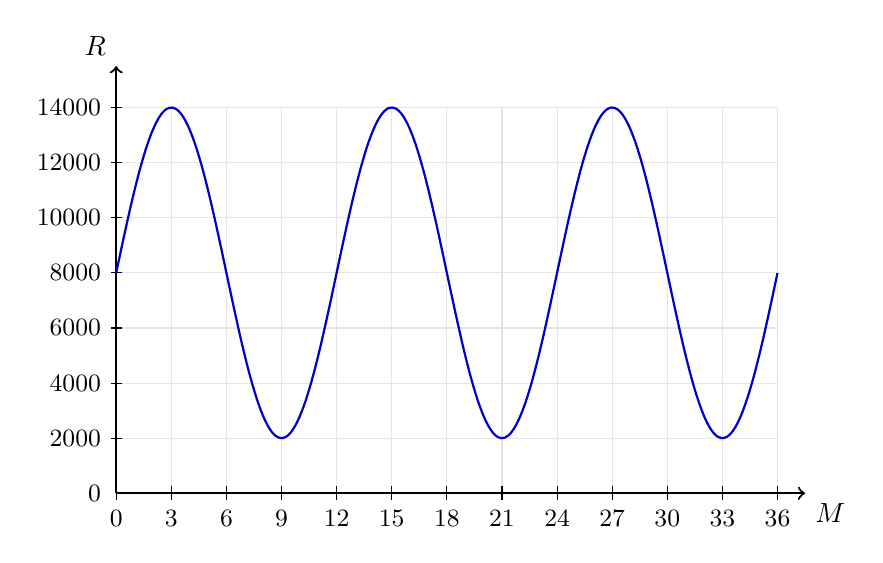
\begin{tikzpicture}[xscale=0.2333, yscale=0.35]
    % Grid lines (horizontal)
    \draw[gray!20, line width=0.4pt] (0,2) -- (36,2);
    \draw[gray!20, line width=0.4pt] (0,4) -- (36,4);
    \draw[gray!20, line width=0.4pt] (0,6) -- (36,6);
    \draw[gray!20, line width=0.4pt] (0,8) -- (36,8);
    \draw[gray!20, line width=0.4pt] (0,10) -- (36,10);
    \draw[gray!20, line width=0.4pt] (0,12) -- (36,12);
    \draw[gray!20, line width=0.4pt] (0,14) -- (36,14);

    % Grid lines (vertical)
    \foreach \x in {0, 3, 6, 9, 12, 15, 18, 21, 24, 27, 30, 33, 36} {
        \draw[gray!20, line width=0.4pt] (\x,0) -- (\x,14);
    }

    % Axes
    \draw[->, thick] (0,0) -- (37.5,0) node[below right] {$M$};
    \draw[->, thick] (0,0) -- (0,15.5) node[above left] {$R$};

    % Y-axis ticks and labels
    \foreach \y/\label in {2/2000, 4/4000, 6/6000, 8/8000, 10/10000, 12/12000, 14/14000} {
        \draw (0.3,\y) -- (-0.3,\y) node[left] {\small\label};
    }
    \node[left] at (-0.3,0) {\small 0};

    % X-axis ticks and labels (3 years / 36 months)
    \foreach \x in {0, 3, 6, 9, 12, 15, 18, 21, 24, 27, 30, 33, 36} {
        \draw (\x, 0.25) -- (\x, -0.25) node[below] {\small\x};
    }

    % Plot the Sine Curve R = 6*sin(30*M) + 8
    \draw[smooth, thick, blue!80!black, domain=0:36, samples=200] 
        plot (\x, {6*sin(30*\x) + 8});
\end{tikzpicture}
\end{center}

\begin{enumerate}
    \item According to the equation, what is the latte revenue in October 2026?  Indicate the point on the graph that shows the answer.
    \item According to the graph, what is the highest latte revenue and in which month of the year does it occur? Explain why your answer makes sense.
    \item According to the graph, what is the lowest latte revenue and in which month does it occur? Explain why your answer makes sense. 
    \item According to the graph, what is the period of this sine model and what does it mean in the story? 
    \item How could we calculate the period of this sine model from the equation?
    \item If we were to include iced latte sales, how do you think the graph would change?  Note: iced latte's are lovely when it's hot out!
\end{enumerate}

\item %workbook 3
Inside a car's engine, controlled micro-explosions of gasoline push a metal cylinder called a piston up and down. The piston's movement turns these explosions into rotational force that powers the vehicle's wheels.  When a car is parked with its engine running (idling) the height, $H$ cm, of the middle of the piston (above the base) is given by the equation
$$H=4 \sin(4500S) + 10$$
where $S$ is the time since the car started, measured in seconds and the sine function is set to take inputs in degrees.

\begin{enumerate}
    \item The car's engine run at $750\text{ RPM}$ which means revolutions (or up/down cycles) per minute.  Convert the units to explain why the car's engine runs at 12.5 cycles per second.
    \item How many seconds does it take for the piston to complete it's up/down cycle? This number is the period of the sine function.  Hint: it's less than 1 second.
    \item Which number in the equation is used to calculate the period?  Check that the period you calculate from the equation equals your answer from part (c).
    \item What does the constant 10 mean in the story and what are its units?
    \item What does the 4 mean in the story and what are its units?
    \item Draw a graph showing the height of the piston for the first 1 second.  
    \item Explain how to see 10, 4, and .08 on the graph.
\end{enumerate}


\item %workbook 4

Ocean tides force seawater to flow back and forth through a narrow opening into a bay. At midnight on Monday, the water reached ``slack tide'', momentarily stopping before it began flowing inward. The water's speed (measured in knots) changes continuously: positive values mean water is rushing into the bay, while negative values mean water is flowing out toward the ocean. The water reaches a maximum inward speed of $+4\text{ knots}$, drops back to $0\text{ knots}$ at slack tide, reaches a peak outward speed of $-4\text{ knots}$, and then returns to $0\text{ knots}$ to repeat the process. This complete back-and-forth cycle repeats every 12 hours and 25 minutes. 

This water flow can be modeled with a sine equation where 
$$H = \text{time (hours since midnight)} \sim \text{indep}$$
$$S = \text{water's speed (knots)} \sim \text{dep}$$
and the sine function is set to take inputs in degrees.

\begin{enumerate}
    \item According to the story, what is the midline of the sine model?  Hint: it occurs at the slack tide.
    \item According to the story, what is the amplitude of the sine model?
    \item According to the story, what is the period of the sine model?
    \item Convert 12 hours and 25 minutes to decimal hours.
    \item Write an equation showing how the water's speed varies over time.  Hint: You will need to use the number 360 and your answer to (d) to find the constant multiplying $H$ in the equation.
\end{enumerate}

\item A community food bank experiences seasonal shifts in weekly volunteer hours. Starting on October 1, volunteer participation begins to pick up, rising to a high around January 1 then dipping to its lowest values around July 1.  Volunteer participation $V$ hours/week is a function of the time of year, $M$ measured in months since October 1. It can be modeled with a sine function whose inputs are in degrees. The equation is
$$V = 70 \sin(30M) + 150$$
Here's a graph of this function for three years.

\begin{center}
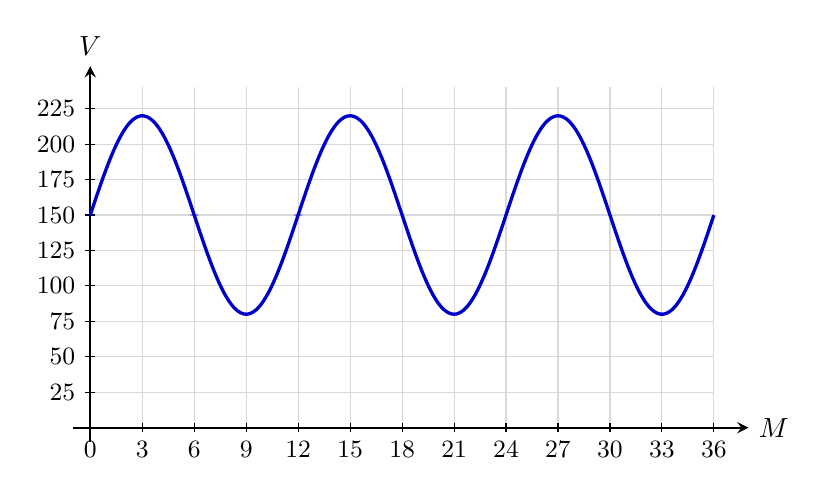
\begin{tikzpicture}[xscale=0.22, yscale=0.018]
    % Vertical Graph Paper Lines (Every 3 months from M = 0 to 36)
    \foreach \x in {0, 3, 6, 9, 12, 15, 18, 21, 24, 27, 30, 33, 36} {
        \draw[gray!30, thin] (\x, 0) -- (\x, 240);
    }

    % Horizontal Graph Paper Lines (At all specified V values)
    \foreach \y in {25, 50, 75, 100, 125, 150, 175, 200, 225} {
        \draw[gray!30, thin] (0, \y) -- (36, \y);
    }
    
    % Main Axes
    \draw[-stealth, thick] (-1,0) -- (38,0) node[right] {$M$};
    \draw[-stealth, thick] (0,-10) -- (0,255) node[above] {$V$};
    
    % X-axis Ticks & Labels (Every 3 months)
    \foreach \x in {0, 3, 6, 9, 12, 15, 18, 21, 24, 27, 30, 33, 36} {
        \draw (\x, 3) -- (\x, -3) node[below, font=\small] {\x};
    }
    
    % Y-axis Ticks & Labels (Including 25, 75, 125, 175, 225)
    \foreach \y in {25, 50, 75, 100, 125, 150, 175, 200, 225} {
        \draw (0.3, \y) -- (-0.3, \y) node[left, font=\small] {\y};
    }
    
    % Sine Curve for 36 months (3 full cycles)
    % Equation: V = 70*sin(30*M) + 150
    \draw[very thick, blue!80!black, smooth, domain=0:36, samples=200]
        plot (\x, {70*sin(30*\x) + 150});
        
    % Key Points Highlighted (Peaks, Troughs, Midline points for Year 1)
    \foreach \x/\y in {0/150, 3/220, 6/150, 9/80, 12/150} {
        \fill[blue!80!black] (\x, \y) circle (8pt);
    }
\end{tikzpicture}
\end{center}

\begin{enumerate}
    \item Use the equation to calculate the volunteer participation at $M=0$, $M=3$, $M=6$, $M=9$, and $M=12$.
    \item According to the graph, what's the highest level of volunteer participation and in what month does that occur? 
    \item Use your equation to determine the highest level of volunteer participation.
    \item According to the graph, what's the lowest level of volunteer participation and in what month does that occur?
    \item Use your equation to determine the lowest level of volunteer participation.
    \item According to the graph, what is the average number of volunteer hours?
    \item Use your equation to determine the average level of volunteer participation.
\end{enumerate}


\item On the shore of a large lake, a sensor on a dock measures the water height. As lake waves pass through, the water level rises above and drops below the average. An equation modeling this phenomenon is
$$ W = 2.5 \sin(60T) + 12 $$
where
$$ W = \text{water height (in feet)} \sim \text{dep} $$
$$ T = \text{time (in seconds)} \sim \text{indep} $$
and the sine function is set to take inputs in degrees.
\begin{enumerate}
    \item What does the constant 12 mean in the story and what are its units?
    \item What does the 2.5 mean in the story and what are its units?
    \item How fast do the waves come? Hint: compute the period. Don't forget the units.
    \item Draw a graph showing the water height for the first minute. Hint: that means up to 60 seconds.
    \item Explain how to see 12, 2.5, and the period in the graph.
\end{enumerate}

\item A warehouse maintains an average inventory of $500\text{ units}$. Deliveries and demand cause stock to fluctuate smoothly between a maximum capacity of $800\text{ units}$ and a low of $200\text{ units}$. At $0\text{ weeks}$, inventory is right at $500\text{ units}$ and rising following a new shipment cycle. The inventory cycle repeats every $4\text{ weeks}$.  The inventory can be modeled with a sine equation where
$$N = \text{ inventory (units) } \sim \text{ dep}$$
$$W = \text{ time (weeks) } \sim \text{ indep}$$
and the sine function is set to take inputs in degrees.

\begin{enumerate}
    \item According to the story, what's the midline of the sine model?
    \item According to the story, what's the amplitude of the sine model?
    \item According to the story, what's the period of the sine model?
    \item Write an equation showing how the inventory varies over time.  Hint: You will need to use the number 360 and your answer to (c) to find the constant multiplying $T$ in the equation.
\end{enumerate}

% \item For John  (like piston) Hobbies: Sewing Machine Needle Position: A sewing machine needle moves vertically relative to the fabric plate. Its midpoint position is $15\text{ mm}$ above the plate, reaching a max height of $25\text{ mm}$ and penetrating down to $5\text{ mm}$. At $t = 0\text{ seconds}$, the needle passes through $15\text{ mm}$ going up. At standard speed ($10\text{ stitches/second}$, period $= 0.1\text{ sec}$), one full cycle takes $0.1\text{ seconds}$.Equation: $h(t) = 10 \sin(3,600t) + 15$


\end{enumerate}

\bigskip

\noindent \textbf{When you're done \ldots}

\begin{itemize}
\item Don't forget to check your answers with those in the back of the textbook. 
\item Not sure if your answers are close enough? Compare with a classmate or ask the instructor.  
\item Getting the wrong answers or stuck on a problem?  Re-read the section and try the problem again.   If you're still stuck, work with a classmate or go to your instructor's office hours.
\item It's normal to find some parts of some problems difficult, but if all the problems are giving you grief, be sure to talk with your instructor or advisor about it.  They might be able to suggest strategies or support services that can help you succeed.
\item Make a list of key ideas or processes to remember from the section.  The ``Do you know?'' questions can be a good starting point.
\end{itemize}



